% chktex-file 44

\cleardoublepage%

\chapter{Modelización estructural}%
\label{makereference5}

Una vez obtenidos tanto los datos de las señales de la infraestructura operacional y la información del entorno del mercado, es necesario realizar un modelado estructural del entrono a optimizar para, tomadas las entradas, determinar la posición del mercado óptima de las baterías.

Exactamente, el objetivo principal de la etapa de optimización del sistema es responder a las cuestiones de cuándo y de qué fuente ciclar energía y cuánta energía ciclar, buscando siempre los mayores ingresos.

Para ello, se ha elegido Pyomo~\cite{pyomo2025optimization} como herramienta de modelización matemática en el área de investigación operacional. Pyomo es una biblioteca de Python para formular, solucionar y analizar problemas de optimización, como el propio.

Se hace uso de una formulación de \gls{milp} para poder tener en cuenta condiciones más allá de la más simple \gls{lp}. Se ha explorado el uso de indicadores o restricciones avanzadas, como los \textit{special order sets}, los cuales han sido descartados en última instancia debido a problemas de rendimiento. Esto significa que la modelización es puramente de enteros mixta compatible con cualquier resolutor que soporte variables binarias.

De esta forma, se detallan los parámetros de decisión en la sección~\ref{makereference5.1}, que articulan el problema de optimización, abarcando desde la definición temporal de los periodos del mercado y las variables de operación de los flujos energéticos, hasta las limitaciones impuestas por el comportamiento físico de la batería y las guías estratégicas de las indicaciones de mercado. Se procede a formular las restricciones operacionales que aseguran la viabilidad técnica de la solución en la sección~\ref{makereference5.2}, se establece el criterio de desempeño que define la función objetivo a optimizar en la parte~\ref{makereference5.3} y, finalmente, se consideran los requisitos de la resolución numérica para cumplir con la precisión exigida por el operador del mercado en la sección~\ref{makereference5.4}.

% TODO
\begin{figure}
  \centering
  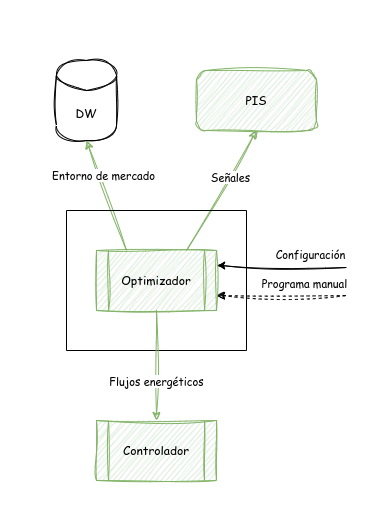
\includegraphics[height=0.75\textheight]{figures/arquitectura-modelizacion.png}
  \caption[Arquitectura de la modelización estructural.]{Arquitectura de la modelización estructural.}%
  \label{fig:arquitectura-modelizacion}
\end{figure}

\section{Parámetros de decisión}%
\label{makereference5.1}

Todo modelado estructural debe contar inicialmente con un conjunto de parámetros de decisión que determinen los valores con los que trabaja el modelo. Más adelante, dichos parámetros son usados para definir las restricciones que el control de la batería debe cumplir.

\subsection{Periodos del mercado}%
\label{makereference5.1.1}

El mercado eléctrico peninsular opera en etapas discretas temporales con una granularidad establecida. Los mercados spot, de los que se encarga el sistema en la actualidad, disponen de una granularidad horaria para el mercado diario\footnote{La granularidad del mercado diario se encuentra en proceso de actualización a cuartohoraria.} y cuartohoraria para los mercados intradiarios y el mercado intradiario continuo. En el resto de mercados de Europa, como Nord Pool~\cite{nord2025leading}, la granularidad de los mercados spot es similar, existiendo también granularidades incluso de 30 minutos.

La variabilidad de la granularidad exige representar el mercado en múltiples periodos categóricos de tamaño proporcional. De esta forma, el sistema representa el mercado mismo mediante la ecuación~\ref{eq:set-mercado}.

\begin{samepage}

  \begin{equation}%
    \label{eq:set-mercado}
    T = \{t_{1} + k \cdot \Delta t \mid k \in \mathbb{R}^{+}_{0}, t_{1} + k \cdot \Delta t \leq t_{1} + H\}
  \end{equation}

  donde

  \begin{itemize}

    \item \( t_{1} \) es el periodo inicial de optimización\footnote{Los periodos son oficialmente representados a partir del índice 1}.

    \item \( \Delta t \) es la granularidad mínima de los mercados analizados dentro del horizonte de optimización en \si{\minute}.

    \item \( H \) es el horizonte de optimización correspondiente al número de días de mercado a tener en cuenta.

    \item \( T \) es el conjunto de todos los períodos de mercado discretos.

  \end{itemize}

\end{samepage}

La representación del mercado durante la optimización realmente incluye multiples posibles mercados futuros más allá del más próximo, es decir, el sistema tiene en cuenta un horizonte de optimización de varios mercados y, por lo tanto, varios periodos a lo largo de múltiples días de mercado. La razón de lo cual reside en facilitar a la optimización la mayor información posible: si un día de mercado no cumple con las condiciones de actuación mientras que otro día de mercado las dobla, es posible no arbitrar uno de los días y ofertar el doble el otro, en vez de perder la oportunidad.

También es necesario tener en cuenta los husos horarios a la hora de calcular el tamaño del mercado, ya que los mercados hacen uso del huso horario local en todo momento, a diferencia de UTC, subrayado anteriormente en la sección~\ref{makereference4.4}. Esto significa que en los días de cambio de hora, los mercados  tendrán más o menos periodos e incluso el mercado intradiario continuo tendrá más o menos sesiones, dependiendo de si se añaden o restan horas. El \gls{mo} lo detalla en verano en la tabla~\ref{tab:cambio-hora-verano} e invierno en la tabla~\ref{tab:cambio-hora-invierno}.

\begin{table}[ht]
  \centering
  \resizebox{\textwidth}{!}{%
    \begin{tabular}{|l|c|c|c|}
      \hline
      & Sesión 1ª & Sesión 2ª & Sesión 3ª                                                                                \\
      \hline
      Apertura de sesión                            & 14:00               & 21:00               & 09:00                  \\
      Cierre de sesión                              & 15:00               & 22:00               & 10:00                  \\
      Casación y publicación                        & 15:20               & 22:20               & 10:20                  \\
      Horizonte de programación (periodos horarios) & 23 horas (1--23 D+1) & 23 horas (1--23 D+1) & 12 horas (12--23 D)  \\
      \hline
    \end{tabular}
  }
  \caption[Ajustes del mercado intradiario en cambios de hora de verano.]{Ajustes del mercado intradiario en cambios de hora de verano.}%
  \label{tab:cambio-hora-verano}
\end{table}

\begin{table}[ht]
  \centering
  \resizebox{\textwidth}{!}{%
    \begin{tabular}{|l|c|c|c|}
      \hline
      & Sesión 1ª & Sesión 2ª & Sesión 3ª                                                                                \\
      \hline
      Apertura de sesión                            & 14:00               & 21:00               & 09:00                  \\
      Cierre de sesión                              & 15:00               & 22:00               & 10:00                  \\
      Casación y publicación                        & 15:20               & 22:20               & 10:20                  \\
      Horizonte de programación (periodos horarios) & 25 horas (1--25 D+1) & 25 horas (1--25 D+1) & 12 horas (14--25 D)  \\
      \hline
    \end{tabular}
  }
  \caption[Ajustes del mercado intradiario en cambios de hora de invierno.]{Ajustes del mercado intradiario en cambios de hora de invierno.}%
  \label{tab:cambio-hora-invierno}
\end{table}

\subsection{Flujos de almacenamiento}%
\label{makereference5.1.2}

De esta forma, el mercado es usado para indexar los flujos energéticos explicados en la sección~\ref{makereference3.1} de infraestructura operacional. Estos flujos energéticos representan la operación y, por lo tanto, salida de la optimización. Responden a las preguntas de cuándo y cuánta energía ciclar.

Aún así, ellos solos no bastan para controlar la batería correctamente como tal. Precisamente, conviene más observar estos flujos energéticos no como flujos energéticos mismos, sino como interfaces de compra y venta, correspondientes a las \gls{ufi} explicadas en el apartado~\ref{makereference4}. Realmente, el sistema se encarga de arbitrar en el mercado, por lo que debe operar no solo en la capa de abstracción de flujos energéticos físicos, sino además en la de los movimientos del mercado.

Todo esto sirve para subrayar que los flujos energéticos, desde la perspectiva del mercado, no están únicamente limitados a la dirección de compra para la carga y venta para la descarga. Una \gls{ufi} correspondiente a la importación de energía también es capaz de vender y una de exportación de comprar, solo que la energía en dirección opuesta al flujo energético no puede provenir de la instalación, ya que el flujo energético fisco lo limita. En cambio, debe provenir del resto de la red eléctrica.

Por ejemplo, como se realizan varias sesiones de mercado en un mismo día, puede que el sistema haya prometido vender una cantidad de energía en un periodo de la tarde en el mercado diario. Lamentablemente, una hora antes de tener que exportar toda esa energía casada (en la última sesión del mercado intradiario continuo antes del \textit{delivery}), resulta que las nuevas previsiones meteorológicas indica que, debido a una nube repentina, los paneles fotovoltaicos no van a ser capaces de generar la suficiente energía como para cargar la batería y exportar su energía. Esto genera un desvío en la posición de la batería: no va a ser capaz de otorgar toda la energía prometida y puede resultar penalizada. Por suerte, como se ha explicado, la solución al problema es recomprar la cantidad de energía que le falte al sistema a través de la interfaz de exportación. Como las recompras (y reventas, en el caso contrario) se realizan exclusivamente en el mismo periodo de su correspondiente posición opuesta por definición, la energía no necesita pasar por la interfaz que ha realizado la operación y la instalación puede exportar la energía tranquilamente y suplir la falta al mismo tiempo, sin tener que importan energía a la instalación. La energía que falta será suministrada entonces por el resto de la red eléctrica en nombre de la instalación.

Por lo tanto, los diferentes flujos energéticos son representados de la siguiente forma, correspondientes con los resultados principales de la optimización.

\begin{itemize}

  \item \( E^{n}_{\text{M}, \text{BESS}, t} \in \mathbb{R}^{+}_{0} \) es la energía neta correspondiente al flujo energético físico importado de la red a la batería en \si{{\mega\watt\hour}}.

  \item \( E^{b}_{\text{M}, \text{BESS}, t} \in \mathbb{R} \) es la energía bruta correspondiente a la actividad en el mercado de la interfaz en \si{{\mega\watt\hour}}.

  \item \( E^{c}_{\text{M}, \text{BESS}, t} \in \mathbb{R}^{+}_{0} \) es la energía casada en negociaciones previas que la batería se ha comprometido a importar en \si{{\mega\watt\hour}}.

  \item \( E^{n}_{\text{BESS}, \text{M}, t} \in \mathbb{R}^{+}_{0} \) es la energía neta correspondiente al flujo energético físico exportado de la batería a la red en \si{{\mega\watt\hour}}.

  \item \( E^{b}_{\text{BESS}, \text{M}, t} \in \mathbb{R} \) es la energía bruta correspondiente a la actividad en el mercado de la interfaz en \si{{\mega\watt\hour}}.

  \item \( E^{c}_{\text{BESS}, \text{M}, t} \in \mathbb{R}^{+}_{0} \) es la energía casada en negociaciones previas que la batería se ha comprometido a exportar en \si{{\mega\watt\hour}}.

\end{itemize}

Los flujos netos y casados son no negativos, ya que representan la energía que mueve la instalación, los flujos brutos, en cambio, representan las operaciones en el mercado, que incluyen recompras o reventas en la dirección opuesta a su flujo energético.

\subsection{Flujos de generación}%
\label{makereference5.1.3}

Aunque, la modelización anterior cubra los \glspl{bess} al completo, el sistema se topa con un problema. ¿Cómo se decide cuándo cargar de la red o de la generación?

Las restricciones previas tan solo dibujan un marco aislado, que no tiene en cuenta que la energía importada de la generación es energía que la instalación, a través de la correspondiente interfaz de exportación de la generación, no es capaz de vender porque la carga de la batería se lo impide.

Por lo tanto, es necesario tener en cuenta la generación junto con la batería y realizar una optimización de los flujos energéticos de la instalación conjunta. Introduciendo la generación a los flujos energéticos de la sección~\ref{makereference5.1.2}, la batería no puede ``robar'' energía a la generación, ya que debe existir una armonía conjunta en busca de la maximización del ingreso.

\begin{itemize}

  \item \( E_{\text{RES}, \text{BESS}, t} \in \mathbb{R}^{+}_{0} \) es la energía importada de la generación a la batería en instalaciones híbridas en \si{{\mega\watt\hour}}.

  \item \( E^{n}_{\text{RES}, R} \in \mathbb{R}^{+}_{0} \) es la energía neta correspondiente al flujo energético físico importado de la red a la batería en \si{{\mega\watt\hour}}.

  \item \( E^{b}_{\text{RES}, R} \in \mathbb{R} \) es la energía bruta correspondiente a la actividad en el mercado de la interfaz en \si{{\mega\watt\hour}}.

  \item \( E^{c}_{\text{RES}, R} \in \mathbb{R}^{+}_{0} \) es la energía casada en negociaciones previas que la generación se ha comprometido a importar en \si{{\mega\watt\hour}}.

\end{itemize}

Como la importación de la generación a la batería no pasa por mercado, no es necesario desglosarla en flujos brutos y netos para acomodar una casación inexistente.

\subsection{Indicaciones de mercado}%
\label{makereference5.1.4}

Con las representaciones de los movimientos de energía, el sistema debe ser capaz de guiar la operación de la batería. Es decir, se busca impedir posiciones que, aunque físicamente posibles, no rentabilicen la batería.

Para ello, se definen los parámetros relacionados con el entorno de mercado, con los que se incorporan las informaciones de las predicciones de precio de mercado anteriormente calculadas según la lógica descrita en la sección~\ref{makereference4.1.1}, las previsiones meteorológicas de la sección~\ref{makereference4.3} para las instalaciones híbridas, y las limitaciones de programa de la sección~\ref{makereference4.2.1} que limitan la potencia de los activos.

\begin{itemize}

  \item \( \lambda' \) es el \textit{spread} mínimo objetivo en \si{\text{\euro}\per\mega\watt\hour}, es decir, el mínimo beneficio a obtener por cada unidad energética negociada.

  \item \( \lambda^{M}_{t} \) es el precio de mercado eléctrico en el periodo \( t \) en \si{\text{\euro}\per\mega\watt\hour}, incluyendo tanto precios positivos como negativos.

  \item \( E_{\text{RES}, t} \) es la energía generada por el activo de generación en instalaciones híbridas en el periodo \( t \) en \si{{\mega\watt\hour}}.

  \item \( P^{\text{lim}}_{\text{BESS}, t} \) es la limitación de programa de la batería en el periodo \( t \) en \si{\mega\watt}, generalmente sin acotar para representar su ausencia.

  \item \( P^{\text{lim}}_{\text{RES}, t} \) es la limitación de programa de la generación en el periodo \( t \) en \si{\mega\watt}, generalmente sin acotar para representar su ausencia.

  \item \( P^{\text{lim}}_{t} \) es la limitación de programa de la instalación al completo en el periodo \( t \) en \si{\mega\watt}, pueden darse múltiples limitaciones pueden en un único periodo de mercado.

\end{itemize}

\subsection{Comportamiento físico}%
\label{makereference5.1.5}

Finalmente, toda batería comparte unos comportamientos físicos intrínsecos. Al fin y al cabo, las baterías son sistemas de almacenamiento de energía que permiten ser cargadas para su posterior descarga, pero ¿cómo de rápido pueden ser cargadas y descargadas, cuánto, cuántas veces, etc.?

Precisamente, las señales propiamente configuradas en el \gls{pis}, detalladas en la sección~\ref{makereference3.2}, permite conocer los parámetros operacionales de las batería. Con ellos, es necesario es representarlos simbólicamente para su optimización operativa.

\begin{itemize}

  \item \( P^{c}_{n} \) es la potencia nominal de carga de la batería en \si{\mega\watt}.

  \item \( P^{d}_{n} \) es la potencia nominal de descarga de la batería en \si{\mega\watt}.

  \item \( P_{n} \) es la potencia nominal de la red de la instalación de la batería en \si{\mega\watt}, es decir, el valor estructural global registrada.

  \item \( E_{n} \) es capacidad de almacenamiento de la batería en \si{{\mega\watt\hour}}.

  \item \( \eta^{c} \) es el rendimiento de carga de la batería.

  \item \( \eta^{d} \) es el rendimiento de descarga de la batería.

  \item \( C_{t} \in \mathbb{R}^{+}_{0} \) es la energía cargada por la batería en el periodo \( t \) en \si{{\mega\watt\hour}}, a diferencia de la importada.

  \item \( D_{t} \in \mathbb{R}^{+}_{0} \) es la energía descargada por la batería en el periodo \( t \) en \si{{\mega\watt\hour}}, a diferencia de la exportada.

  \item \( N_{\text{máx}} \) es el número de ciclos máximos a realizar por la batería a lo largo del horizonte de optimización.

  \item \( N \in \mathbb{R}^{+}_{0} \) es el número de ciclos realizados por la batería a lo largo de todo el horizonte de optimización.

  \item \( \text{SoC}_{\text{mín}}, \text{SoC}_{\text{máx}} \) son el \gls{soc} mínimo y máximo de la batería, respectivamente.

  \item \( \text{SoC}_{t} \in \mathbb{R}^{+}_{0} \) es la cantidad de energía almacenada en la batería en el periodo \( t \) en \si{{\mega\watt\hour}}.

  \item \( \text{SoH} \) es el \gls{soh} de la batería, afectando tanto a la potencia y capacidad de almacenamiento.

  \item \( A \) es la disponibilidad de la batería.

\end{itemize}

\section{Restricciones operacionales}%
\label{makereference5.2}

Conociendo los parámetros con trabajar, es momento de definir las restricciones operacionales que establecen las relaciones entre ellos\footnote{Las ecuaciones mostradas se encuentran parcialmente simplificadas para facilitar la comprensión, aunque resulten más robustas en realidad. No se muestran, por ejemplo, las restricciones de consignación manual tanto de la posición como el estado de carga, explicadas en el apartado~\ref{makereference6}}.

Como algunas configuraciones topológicas no soportan todos los flujos energéticos, véase la importación de la red en la topología híbrida con carga aislada de la red o la importación de la generación en la aislada, estas deben ser capaces de ser desactivadas a través de la relación~\ref{eq:desactivación-ufi}.

\begin{samepage}

  \begin{equation}%
    \label{eq:desactivación-ufi}
    E^{n}_{t} =
    \begin{cases}
      E^{n}_{t} & \text{si } \exists \, \text{UFI} \\
      0         & \text{sino}                      \\
    \end{cases}
  \end{equation}

  donde

  \begin{itemize}

    \item \( \text{UFI} \) determina la existencia de la \gls{ufi} correspondiente al flujo energético,  \( \text{UFI}_{\text{BESS}, R} \), \( \text{UFI}_{\text{M}, \text{BESS}} \), \( \text{UFI}_{\text{RES}, \text{BESS}} \) y \( \text{UFI}_{\text{RES}, R} \).

    \item \( E^{n}_{t} \) es la energía importada o exportada de cada flujo energético en \si{{\mega\watt\hour}}, \( E_{\text{BESS}, \text{M}, t} \), \( E_{\text{M}, \text{BESS}, t} \), \( E_{\text{RES}, \text{BESS}, t} \) y \( E_{\text{RES}, \text{M}, t} \).

  \end{itemize}

\end{samepage}

Con esto, los flujos energéticos netos están definidos como la suma del correspondiente flujo energético bruto y el casado, es decir, el flujo energético físico representado por el parámetro neto debe ser siempre no negativo, pero la interfaz de la \gls{ufi} lo puede ser cuando existan posiciones casadas en un periodo concreto. Esto es representado por la ecuación~\ref{eq:neto-bruto} y se realiza para cada uno de los flujos energéticos con \glspl{ufi} arbitrados en el mercado, es decir, para la importación de la red y exportación a la red.

\begin{samepage}

  \begin{equation}%
    \label{eq:neto-bruto}
    E^{n}_{t} = E^{b}_{t} + E^{c}_{t}
  \end{equation}

  donde

  \begin{itemize}

    \item \( E_{t} \) es la energía importada o exportada de cada flujo energético desde o a la red en \si{{\mega\watt\hour}}, \( E_{\text{BESS}, \text{M}, t} \), \( E_{\text{M}, \text{BESS}, t} \) y \( E_{\text{RES}, \text{M}, t} \).

  \end{itemize}

\end{samepage}

Con respecto a los parámetros del comportamiento físico, estos limitan la potencia tanto de carga como de descarga\footnote{Aunque la potencia de carga y descarga generalmente coincida en las instalaciones para las que se ha desplegado el sistema, es importante reconocer que pueden no ser iguales.}, mediante la ecuación~\ref{eq:capacidad-potencia-carga} de carga y la ecuación~\ref{eq:capacidad-potencia-descarga} de descarga. Las señales de disponibilidad y \gls{soh} afectan linealmente a la capacidad de potencia: para una disponibilidad o \gls{soh} de la mitad, la potencia de la batería es la mitad de su capacidad nominal.

\begin{equation}%
  \label{eq:capacidad-potencia-carga}
  C_{t} \le A \cdot \text{SoH} \cdot P^{c}_{n} \cdot \Delta t
\end{equation}

\begin{equation}%
  \label{eq:capacidad-potencia-descarga}
  D_{t} \le A \cdot \text{SoH} \cdot P^{d}_{n} \cdot \Delta t
\end{equation}

Junto a la potencia, la capacidad de almacenamiento la limita el correspondiente parámetro nominal de la batería en~\ref{eq:capacidad-almacenamiento}.

\begin{equation}%
  \label{eq:capacidad-almacenamiento}
  \text{SoC}_{t} \le A \cdot \text{SoH} \cdot E_{n}
\end{equation}

Las eficiencias de carga y descarga también afectan al ciclado, incorporadas en los respectivos cálculos de la energía cargada y descargada. Para ello, resulta absolutamente necesario separar la carga por un lado y la descarga por el otro, ya que el cálculo del número de ciclos del \gls{kpi} correspondiente requiere el uso de la descarga por separado. Como se indica oficialmente, ``se completa un ciclo de carga cuando se ha usado (descargado) una cantidad equivalente al 100 \% de la capacidad de la batería, pero no necesariamente toda con una sola carga. Por ejemplo, se puede usar el 75 \% de la capacidad de la batería un día y luego recargarla completamente durante la noche. Si se usa el 25 \% al día siguiente, se habrá descargado el 100 \% en total, y los dos días sumarán un ciclo de carga''~\cite{apple2025batteries}.

Esto significa que, si la carga y la descarga no se separasen, el número de ciclos sería contado incorrectamente, causados por transiciones que dejasen la batería en el mismo estado. De esta forma, las ecuaciones de las eficiencias detallan la carga proveniente tanto de la importación de la red y de la importación de la generación en~\ref{eq:eficiencia-carga}, y la descarga en~\ref{eq:eficiencia-descarga}.

\begin{equation}%
  \label{eq:eficiencia-carga}
  C_{t} = \eta^{c} \cdot (E^{n}_{\text{M}, \text{BESS}, t} + E_{\text{RES}, \text{BESS}, t})
\end{equation}

\begin{equation}%
  \label{eq:eficiencia-descarga}
  D_{t} = {(\eta^{d})}^{-1} \cdot E^{n}_{\text{BESS}, \text{M}, t}
\end{equation}

Aún así, separar la carga y la descarga directamente introduce uno de los mayores posibles problemas del sistema, la carga y descarga simultanea, detallada más profundamente en la sección~\ref{makereference6.1.1}. Para evitar esta situación, se introducen variables binarias en la formulación~\ref{eq:carga-descarga-simultanea}, que indican la dirección de la operación en la que se encuentra la batería en un periodo determinado, impidiendo así el solapamiento de la carga y descarga. Con el uso de las variables binarias, se reformula la decisión no lineal en sistemas de ecuaciones lineales.

\begin{subequations}%
  \label{eq:carga-descarga-simultanea}

  \begin{equation}
    C_{t} \le M^{\text{c}}_{t} \cdot z^{\text{c}}_{t}
  \end{equation}

  \begin{equation}
    D_{t} \le M^{\text{c}}_{t} \cdot (1 - z^{\text{c}}_{t})
  \end{equation}

  donde

  \begin{itemize}

    \item \( M^{\text{c}}_{t} = E_{n} \) es la cota superior de la máxima carga o descarga permitida en el periodo \( t \) en \si{{\mega\watt\hour}}.

    \item \( z^{\text{c}}_{t} \) es la variable binaria indicador que representa la dirección de carga o descarga en el periodo \( t \).

  \end{itemize}

\end{subequations}

Con ello, un aspecto a tener en cuenta es la simplificación de la formulación mediante \textit{special order sets} de orden 1, y evitar así el uso de variables binarias, como se indica en la ecuación~\ref{eq:carga-descarga-simultanea-sos}.

\begin{equation}%
  \label{eq:carga-descarga-simultanea-sos}
  C_{t}, D_{t} \in \text{SOS}_{1}
\end{equation}

Los \textit{special order sets} permiten representar condiciones de exclusión, tan solo permitiendo la activación (\( > 0 \)) de un número de variables contiguas según su orden, manteniendo el resto desactivadas (\( = 0 \)). En este caso, se pueden usan los \textit{special order sets} de orden 1 para, entre la carga y descarga, activar únicamente una de ellas.

Si las variables de carga y descarga no estuvieran limitadas físicamente (cota superior indefinida), el uso de cotas superiores arbitrariamente altas para satisfacer la restricción de enteros mixta podría afectar negativamente al rendimiento del sistema\footnote{Es posible introducir problemas de estabilidad numérica causados al manipular parámetros de magnitudes comparativamente grandes.}. Sin embargo, como en la formulación planteada no existen dichos problemas, se sigue optando por la solución más extendida de enteros mixta.

El parámetro de mercado de ciclos máximos limita los ciclos a realizar durante el horizonte de optimización, mediante la ecuación~\ref{eq:limite-ciclos}. Inteligentemente, con el proposition de evitar la introducción de relaciones no lineales causadas por mantener un cupo diario de ciclos, se agregan todos ellos a lo largo del horizonte de optimización, en la ecuación~\ref{eq:limite-ciclos-dia}.

\begin{equation}%
  \label{eq:limite-ciclos}
  N \le N_{\text{máx}}
\end{equation}

\begin{samepage}

  \begin{equation}%
    \label{eq:limite-ciclos-dia}
    N_{\text{máx}} = N_{d} \cdot H
  \end{equation}

  donde

  \begin{itemize}

    \item \( N_{d} \) es el número de ciclos máximos a realizar por la batería por día.

  \end{itemize}

\end{samepage}

A su vez, el cálculo de los ciclos totales se define en la ecuación~\ref{eq:ciclado}, tan solo teniendo en cuenta la energía descargada.

\begin{equation}%
  \label{eq:ciclado}
  N = \sum_{t = 1}^{H} D_{t} \cdot E_{n}^{-1}
\end{equation}

Por otro lado, el \gls{soc} lo limitan las señales de la batería en la ecuación~\ref{eq:limite-soc}. Generalmente, se suele reservar un margen de 5--10 \% de la capacidad de almacenamiento nominal para evitar imprevistos.

Precisamente, un efecto secundario muy beneficioso de las limitaciones de la señal del \gls{soc} es la posibilidad de la participación de las baterías en los mercados de disponibilidad\footnote{El sistema no soporta los mercados de disponibilidad en su estado actual, aunque sí que permite manejarlos externamente.}. Como en ningún momento se llega ni al máximo ni al mínimo de la capacidad de la batería, esta puede ofertar por lo menos el rango del \gls{soc} a subir o bajar y generar beneficios pasivos, sin afectar de ninguna forma a la operación principal en los mercados spot.

\begin{subequations}%
  \label{eq:limite-soc}

  \begin{equation}
    \text{SoC}_{t} \ge \text{SoC}_{\text{mín}} \cdot E_{n}
  \end{equation}

  \begin{equation}
    \text{SoC}_{t} \le \text{SoC}_{\text{máx}} \cdot E_{n}
  \end{equation}

\end{subequations}

De esta forma, se define la ecuación del \gls{soc}~\ref{eq:soc}, teniendo en cuenta la energía cargada y descargada.

\begin{equation}%
  \label{eq:soc}
  \text{SoC}_{t} = \text{SoC}_{t - 1} + C_{t} - D_{t}
\end{equation}

Además, la modelización también debe tener en cuenta las limitaciones de programa obtenidas en la sección~\ref{makereference4.2.1}. Estas limitaciones, representadas en la ecuación~\ref{eq:limite-programa}, impiden la exportación de energía de cada uno de los activos energéticos individualmente.

\begin{subequations}%
  \label{eq:limite-programa}

  \begin{equation}
    E^{n}_{\text{BESS}, \text{M}, t} \le \min(P_{n}, P^{\text{lim}}_{\text{BESS}, t}) \cdot \Delta t
  \end{equation}

  \begin{equation}
    E^{n}_{\text{RES}, \text{M}, t} \le \min(P_{n}, P^{\text{lim}}_{\text{RES}, t}) \cdot \Delta t
  \end{equation}

  \begin{equation}
    E^{n}_{\text{BESS}, \text{M}, t} + E^{n}_{\text{RES}, \text{M}, t} \le \min(P_{n}, P^{\text{lim}}_{t}) \cdot \Delta t
  \end{equation}

\end{subequations}

Con esto, como las limitaciones de programa son especificas del activo, estas restricciones introducen nuevas oportunidades de arbitraje en instalaciones híbridas, resultado de que generación se vea limitada sin estarlo la exportación de la batería. Ante dicha situación, la batería es capaz de cargarse sin ningún coste.

Para mejorar el rendimiento teniendo en cuenta estas circunstancias, se introducen nuevas restricciones en forma de la ecuación~\ref{eq:curtailed-import}, que controla la importación de energía excedente y la importación de energía no excedente. Concretamente, el termino usado para referirse a la energía excedente que sobrepasa los límites de exportación se conoce como \textit{curtailment}.

\begin{samepage}%
  \label{eq:curtailed-import}

  \begin{equation}%
    E^{\text{c}}_{\text{RES}, \text{BESS}, t} \le
    \begin{cases}
      E_{\text{RES}, t} - \min(P_{n}, P^{\text{lim}}_{\text{RES}, t}) * \Delta t & \text{si } E_{\text{RES}, t} > \min(P_{n}, P^{\text{lim}}_{\text{RES}, t}) * \Delta t \\
      0                                                                          & \text{sino}                                                                           \\
    \end{cases}
  \end{equation}

  \begin{equation}%
    E^{\text{nc}}_{\text{RES}, \text{BESS}, t} \le
    \begin{cases}
      E_{\text{RES}, t}                                      & \text{si } E_{\text{RES}, t} \le \min(P_{n}, P^{\text{lim}}_{\text{RES}, t}) * \Delta t \\
      \min(P_{n}, P^{\text{lim}}_{\text{RES}, t}) * \Delta t & \text{sino}                                                                             \\
    \end{cases}
  \end{equation}

  donde

  \begin{itemize}

    \item \( E^{\text{c}}_{\text{RES}, \text{BESS}, t} \) es la importación de la generación excedente a la batería en \si{{\mega\watt\hour}}.

    \item \( E^{\text{nc}}_{\text{RES}, \text{BESS}, t} \) es la importación de la generación no excedente a la batería en \si{{\mega\watt\hour}}.

  \end{itemize}

\end{samepage}

Junto a estas restricciones, se debe impedir la importación de energía no excedente cuando la excedente se encuentre disponible, lo cual puede ocurrir cuando existen limitaciones de programa o los precios de mercado sean nulos o negativos. Por ello, se añade otra restricción indicativa de enteros mixta a la formulación, ecuación~\ref{eq:indicador-curtailment}.

\begin{subequations}%
  \label{eq:indicador-curtailment}

  \begin{equation}
    E^{\text{c}}_{\text{RES}, \text{BESS}, t} \le M^{\text{nc}}_{t} \cdot z^{\text{nc}}_{t}
  \end{equation}

  \begin{equation}
    E^{\text{nc}}_{\text{RES}, \text{BESS}, t} \le M^{\text{nc}}_{t} \cdot (1 - z^{\text{nc}}_{t})
  \end{equation}

  donde

  \begin{itemize}

    \item \( M^{\text{nc}}_{t} = E_{\text{RES}, t} \) es la cota superior de la máxima importación de generación disponible en el periodo \( t \) en \si{{\mega\watt\hour}}.

    \item \( z^{\text{nc}}_{t} \) es la variable binaria indicador que representa el estado de la importación excedente de la generación a la batería en el periodo \( t \), es decir, si se está cargando de la energía excedente o no.

  \end{itemize}

\end{subequations}

La introducción del desglose de la importación de la generación a la batería significa que la importación misma debe estar definida según la ecuación~\ref{eq:res-import}.

\begin{equation}%
  \label{eq:res-import}
  E_{\text{RES}, \text{BESS}, t} = E^{\text{c}}_{\text{RES}, \text{BESS}, t} + E^{\text{nc}}_{\text{RES}, \text{BESS}, t}
\end{equation}

A su vez, se dispone de toda la información necesaria para completar el cálculo de la posición de venta de la generación, ya que, tal y como se ha descrito anteriormente, es necesario optimizar tanto el ciclado de la batería, como la venta de la generación, para obtener una visión completa del movimiento de la instalación. Con ello, la exportación de la generación en la ecuación~\ref{eq:res-export} se corresponde con la venta de todo el recurso generado del que no ha cargado la batería, limitado por los limites de programa y limitaciones estructurales.

\begin{equation}%
  \label{eq:res-export}
  E^{n}_{\text{RES}, \text{M}, t} =
  \begin{cases}
    E^{n}_{\text{RES}, t} - E^{\text{nc}}_{\text{RES}, \text{BESS}, t} & \text{si } E_{\text{RES}, t} \le \min(P_{n}, P^{\text{lim}}_{\text{RES}, t}) \cdot \Delta t \\
    \min(P_{n}, P^{\text{lim}}_{\text{RES}, t}) * \Delta t - E^{\text{nc}}_{\text{RES}, \text{BESS}, t} & \text{sino}                                                \\
  \end{cases}
\end{equation}

Con esto, aunque las relaciones definidas son aplicables a la importación de la generación propia de las instalaciones híbridas, estas muestran comportamientos variados más allá de la configuración híbrida flexible, descritos en la sección~\ref{makereference3.1.2}.

Precisamente, para adecuarse a los de la configuración híbrida con carga aislada de la red, se introduce el concepto de \textit{clipping}. El \textit{clipping} es un comportamiento en donde se restringe la carga de la batería únicamente a la generación excedente\footnote{Los coeficientes de \textit{clipping} se han calculado inicialmente con la consulta de las especificaciones de la instalación y han sido posteriormente refinados mediante \textit{backtesting}, gracias al trabajo previo realizada mediante consultas del \gls{pis}.}, representado en la figura~\ref{fig:clipping}.

A modo de analogía, el \textit{clipping} se puede entender como una persona que dispone de un salario fijo (generación). Cada mes debe pagar una cantidad de su salario para el alquiler (\textit{threshold} de carga). Del dinero sobrante, ahorra (carga) una porcentaje (coeficiente de \textit{clipping}), mientras que gasta el resto como le apetezca (exportación de generación). Se representa mediante la ecuación~\ref{eq:clipping}.

\begin{figure}
  \centering
  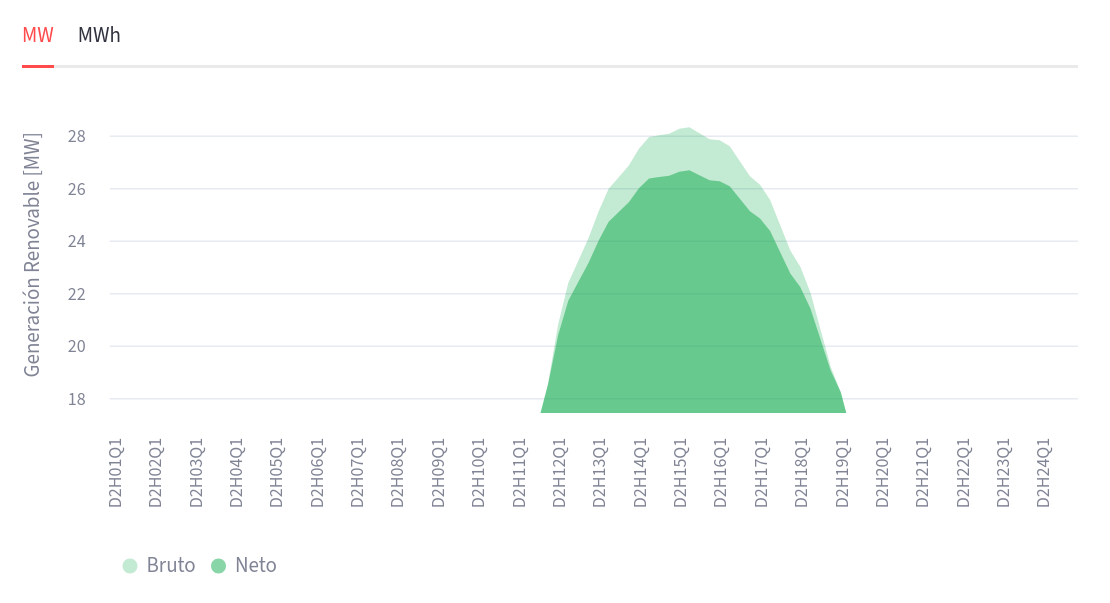
\includegraphics[width=0.75\linewidth]{figures/clipping.png}
  \caption[Clipping de configuración topológica híbrida.]{Clipping de la configuración topológica híbrida con carga aislada de la red. La batería solo es capaz de cargar del excedente porcentual de generación, dibujando una curva de carga en los picos.}%
  \label{fig:clipping}
\end{figure}

\begin{samepage}

  \begin{equation}%
    \label{eq:clipping}
    E_{\text{RES}, \text{BESS}, t} =
    \begin{cases}
      \gamma * (E_{\text{RES}, t} - \gamma_{\text{u}} * \Delta t) & \text{si } E_{\text{RES}, t} > \gamma_{\text{u}} * \Delta t \\
      0                                                           & \text{sino}                                                 \\
    \end{cases}
  \end{equation}

  donde

  \begin{itemize}

    \item \( \gamma \) es el coeficiente de \textit{clipping} que indica la cantidad de energía excedente con respecto a la generación total.

    \item \( \gamma_{\text{u}} \) es el umbral de \textit{clipping} en \si{\mega\watt}, es decir, la cantidad mínima de energía a partir de la cual considerar excedente.

  \end{itemize}

\end{samepage}

La última configuración topológica a tener en cuenta se trata de la híbrida con prioridad de carga de generación. Esto significa que se debe agotar completamente el recurso de generación antes de poder cargar de la red, aunque cargar de la red otorgue mayores beneficios, como es el caso con los precios de mercado negativos.

Dicha prioridad es definida de forma simular a previas restricciones de indicación con una formulación de enteros mixta en la ecuación~\ref{eq:prioridad-hibrida}. La restricción permanece inactiva si la topología de la instalación (a través de la \gls{ufi}) no se adecua con la híbrida con prioridad de carga de generación.

\begin{subequations}%
  \label{eq:prioridad-hibrida}

  \begin{equation}
    E^{n}_{\text{RES}, \text{M}, t} \le M^{\text{p}}_{t} \cdot z^{\text{p}}_{t}
  \end{equation}

  \begin{equation}
    E^{n}_{\text{M}, \text{BEES}, t} \le M^{\text{c}}_{t} \cdot (1 - z^{\text{p}}_{t})
  \end{equation}

  donde

  \begin{itemize}

    \item \( M^{\text{p}}_{t} = E_{\text{RES}, t} \) es la cota superior de la máxima exportación de generación disponible en el periodo \( t \) en \si{{\mega\watt\hour}}.

    \item \( M^{\text{c}}_{t} = E_{n} \) es la cota superior de la máxima importación máxima permitida por la batería en el periodo \( t \) en \si{{\mega\watt\hour}}.

    \item \( z^{\text{p}}_{t} \) es la variable binaria indicador que representa el estado de prioridad en el periodo \( t \), es decir, si se ha llegado a agotar el recurso de generación o si todavía está disponible.

  \end{itemize}

\end{subequations}

Como se puede observar, el sistema es completamente genérico e incorpora comportamientos generales, a diferencia de definir entidades separadas para cada configuración. Es decir, la lógica base de la optimización no varía segun la configuración.

\section{Criterio de desempeño}%
\label{makereference5.3}

Como se ha mencionado en múltiples ocasiones, el criterio de desempeño del sistema parece ser el beneficio obtenido, es decir, que el sistema busque maximizar los ingresos, en cambio, esto no es del todo cierto.

Inicialmente, en el beneficio toma parte cada flujo de energía. Importantemente, como el sistema asume que las recompras y reventas se realizan al mismo precio que la posible compra y venta\footnote{En realidad, las recompras y reventas, entendiblemente, se realizan al precio de casación anterior, pero no se dispone de la información necesaria para realizar el desglose entre mercados y obtener el precio.}, tan solo se tienen en cuenta las energías netas, correspondientes a los flujos físicos, para el calculo de los ingresos. Con ello, se le asigna un precio a cada uno de ellos, resultando en la ecuación~\ref{eq:beneficio}.

\begin{subequations}%
  \label{eq:beneficio}

  \begin{equation}
    \begin{split}
      \pi_{t}
      = (\lambda^{n}_{\text{BESS}, \text{M}, t} - \lambda')
      \cdot E^{n}_{\text{BESS}, \text{M}, t}\\
      - \lambda^{n}_{\text{M}, \text{BESS}, t}
      \cdot E^{n}_{\text{M}, \text{BESS}, t}\\
      - \lambda^{\text{c}}_{\text{RES}, \text{BESS}, t}
      \cdot E^{\text{c}}_{\text{RES}, \text{BESS}, t}\\
      - \lambda^{\text{nc}}_{\text{RES}, \text{BESS}, t}
      \cdot E^{\text{nc}}_{\text{RES}, \text{BESS}, t}\\
      + \lambda^{n}_{\text{RES}, \text{M}, t}
      \cdot E^{n}_{\text{RES}, \text{M}, t}\\
    \end{split}
  \end{equation}

  \begin{equation}
    \pi = \sum_{t = t_{1}}^{T} \pi_{t}
  \end{equation}

  \begin{equation}
    \lambda^{n}_{\text{BESS}, \text{M}, t} = \lambda^{M}_{t}
  \end{equation}

  \begin{equation}
    \lambda^{n}_{\text{M}, \text{BESS}, t} = \lambda^{M}_{t} + c
  \end{equation}

  \begin{equation}
    \lambda^{\text{c}}_{\text{RES}, \text{BESS}, t} = 0
  \end{equation}

  \begin{equation}
    \lambda^{\text{nc}}_{\text{RES}, \text{BESS}, t} =
    \begin{cases}
      \lambda^{M}_{t} & \text{si } \exists \, \gamma \land \lambda^{M}_{t} \ge \lambda^{O}_{\text{RES}, t} \\
      0               & \text{sino}                                                                        \\
    \end{cases}
  \end{equation}

  \begin{equation}
    \lambda^{n}_{\text{RES}, \text{M}, t} =
    \begin{cases}
      \lambda^{M}_{t} & \text{si } \lambda^{M}_{t} \ge \lambda^{O}_{\text{RES}, t} \\
      0               & \text{sino}                                                \\
    \end{cases}
  \end{equation}

\end{subequations}

donde

\begin{itemize}

  \item \( c \) es el peaje de la red en \si{\text{\euro}\per\mega\watt\hour}.

  \item \( \lambda^{n}_{\text{BESS}, \text{M}, t} \) es el precio de la exportación de la batería a la red en el periodo \( t \) en \si{\text{\euro}\per\mega\watt\hour}.

  \item \( \lambda^{n}_{\text{M}, \text{BESS}, t}\) es el precio de la importación de la red a la batería en el periodo \( t \) en \si{\text{\euro}\per\mega\watt\hour}.

  \item \( \lambda^{O}_{\text{RES}, t} \) es el precio de oferta de la generación en el periodo \( t \) en \si{\text{\euro}\per\mega\watt\hour}.

  \item \( \lambda^{\text{c}}_{\text{RES}, \text{BESS}, t} \) es el precio de la importación de la generación excedente a la batería en el periodo \( t \) en \si{\text{\euro}\per\mega\watt\hour}.

  \item \( \lambda^{\text{nc}}_{\text{RES}, \text{BESS}, t} \) es el precio de la importación de la generación no excedente a la batería en el periodo \( t \) en \si{\text{\euro}\per\mega\watt\hour}.

  \item \( \lambda^{n}_{\text{RES}, \text{M}, t} \) es el precio de exportación de la generación a la red en el periodo \( t \) en \si{\text{\euro}\per\mega\watt\hour}.

  \item \( \pi \) es el beneficio en \si{\text{\euro}}.

\end{itemize}

Si bien la maximización del beneficio es el objetivo principal, el sistema debe tener en cuenta otros factores. De hecho, cuando se realiza la optimización, considerar el beneficio únicamente resulta, casi con total certeza, en un problema de optimización degenerado.

Los problemas de optimización degenerados son los que poseen múltiples soluciones para una misma formulación. El sistema, por el contrario, debe asegurar una optimización estricta (determinista) para facilitar el control de las baterías. No se puede permitir que, ante cualquier modificación en la configuración, por muy minúscula que sea, la posición óptima cambie drásticamente y genere desvíos. La diferencia se observa en la figura~\ref{fig:solucion-degenerada}, en la cual las operaciones de mercado se realizan en periodos incongruentes y se mezclan fuentes de carga, resultado de no acotar con exactitud la optimización\footnote{Se obtiene el mismo resultado del cálculo en múltiples soluciones, aunque verdaderamente solo una de ellas sea la correcta, por lo que el resolutor puede devolver una posición que genere desvíos innecesarios.}.

\begin{figure}
  \centering
  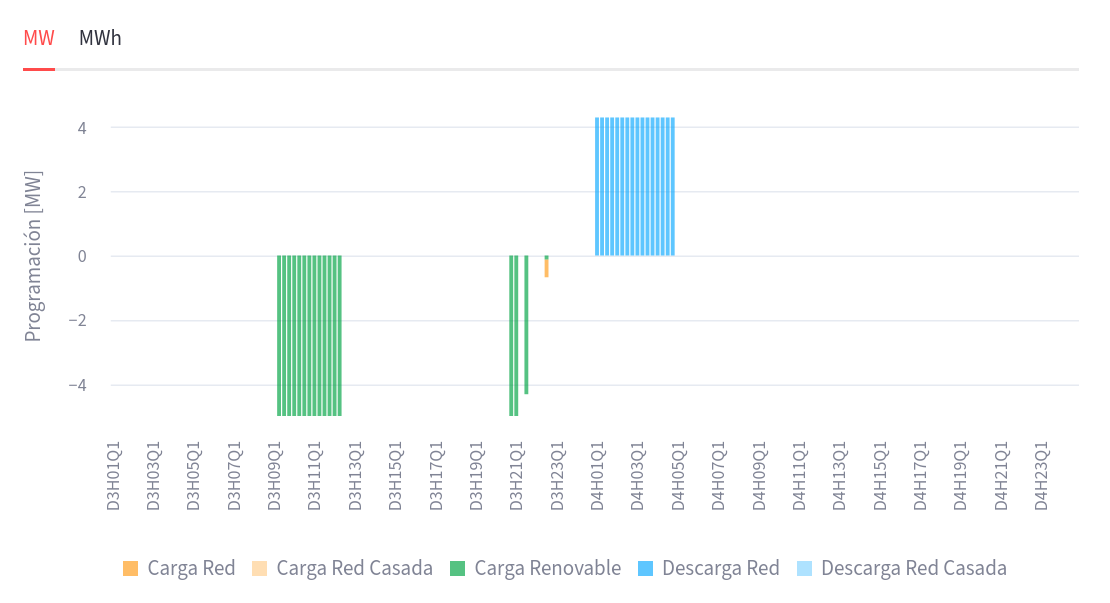
\includegraphics[width=0.75\linewidth]{figures/solucion-degenerada.png}
  \caption[Solución degenerada.]{Solución degenerada a una posición de mercado. Las operaciones se ofertan en periodos inconsistentes, en vez de realizarlas todas en un único bloque desde el primer periodo óptimo (del D3H09Q2 al D3H13Q1 de carga y del D3H22Q4 al D4H01Q4 de descarga). Como también se llevan posiciones al mercado (periodo D3H22Q3) aun no siendo necesario, se generan desvíos.}%
  \label{fig:solucion-degenerada}
\end{figure}

Para solucionar este problema, se tiene en cuenta que las predicciones de precio de mercado y las predicciones meteorológicas, es decir, la información extraída en el apartado~\ref{makereference4} del entorno de mercado, es más precisa cuanto más cercana en el tiempo sea. En otras palabras, las previsiones para el día de mañana resultan más fiables que las de dentro de una semana.

En la formulación, esta preferencia de las posiciones más cercanas en el tiempo se representa con una función de decrecimiento o \textit{decay function} exponencial, ecuación~\ref{eq:exponential-decay}. Dispone de un ratio de decrecimiento configurable dependiente del horizonte de optimización, cuanto mayor sea, menor valor tendrá el ratio de decrecimiento, para evitar conflictos en donde peor posición más cercana en el tiempo sea elegida ante una mejor más lejana.

\begin{samepage}

  \begin{equation}%
    \label{eq:exponential-decay}
    \sum_{t = t_{1}}^{T} e^{-\rho t} \pi_{t}
  \end{equation}

  donde

  \begin{itemize}
    \item \( \rho \) es el coeficiente de decaimiento que favorece los periodos más tempranos.
  \end{itemize}

\end{samepage}

De esta forma, tras realizar el llamado test de factibilidad básica e identificar las variables básicas\footnote{Las variables básicas son las que marcan los puntos extremos de las soluciones, pero no tienen por que encontrarse en su límite, lo cual resultó ser fuente de confusión en el análisis de factibilidad.} y sus propiedades, se determina que la formulación propuesta es estricta.

\subsection{Optimización lexicográfica}%
\label{makereference5.3.1}

Aunque el uso de una función de decrecimiento exponencial distinga correctamente las soluciones de forma determinista, es posible, dependiendo de los parámetros de configuración, que la solución obtenida por el resolutor sea la óptima según el criterio de desempeño definido, pero no la que el sistema busca. Esto sucede debido a que parámetros de decisión incorrectamente seleccionados pueden priorizar una posición que mejore el objetivo de la preferencia temporal y no el del beneficio.

La metodología anterior de juntar los dos objetivos se conoce como optimización multiobjetivo ponderada, donde el coeficiente de ponderación es el calculado mediante la \textit{decay function} exponencial. Aún así, existe una técnica de optimización multiobjetivo más avanzada que evita conflictos entre ellos gracias a una metodología de priorización de objetivos, llamada optimización lexicográfica. Resulta usada esporádicamente incluso en el contexto de los \gls{bess}~\cite{karimi2019multi}.

De esta forma, se desarrolla el algoritmo~\ref{alg:optimizacion-lexicografica} de optimización lexicográfica multiobjetivo por encima del lenguaje de modelado abstracto para asegurar la priorización de los objetivos de la modelización, ya que la herramienta de modelado utilizada no soporta solucionar múltiples objetivos al mismo tiempo.

\begin{algorithm}
  \caption{Algoritmo de optimización lexicográfica}%
  \label{alg:optimizacion-lexicografica}
  \begin{algorithmic}
    \Require{} Funciones objetivo \( f_{1}, \dots, f_{n} \) ordenadas por importancia decreciente.
    \Require{} Variables de decisión \( x \).
    \Require{} Conjunto de valores posibles \( X \).
    \For{\( i \gets 1 \text{ to } n \)}
    \State{} Resolver el problema de optimización de objetivo único \( P_{i} \):
    \Statex{} \hspace{\algorithmicindent} \( \max \quad f_{i}(x) \)
    \Statex{} \hspace{\algorithmicindent} \( \text{sujeto a} \quad x \in X \)
    \Statex{} \hspace{\algorithmicindent} \( \phantom{\text{sujeto a} \quad} f_{j}(x) \geq z_k^* \quad \forall j \in \{1, \dots, i - 1\} \)
    \If{la solución no es factible}
    \State{} \Return{} \( \emptyset \)
    \EndIf{}
    \State{} Sea \( x^{*}_{i} \) una solución óptima para \( P_{i} \).
    \State{} \( z^{*}_{i} \gets f_t(x^{*}_{i}) \) \Comment{Se guarda el valor óptimo para la siguiente iteración.}
    \EndFor{}
    \State{} \Return{} \( x^{*}_{n} \)
  \end{algorithmic}
\end{algorithm}

Con esto, el objetivo principal se trata de la maximización del beneficio y el objetivo secundario la priorización temporal, porque se sigue necesitando obtener una única solución. El sistema permite definir otros objetivos secundarios de menor prioridad, como la maximización del \gls{soc} final para aprovechar situaciones de carga gratuita en las que la energía no es vendida.

Aunque se solucionen los problemas de posiciones posiblemente no óptimas, la optimización lexicográfica tiene un menor rendimiento, por lo que no es factible usarla para mercados con una granularidad muy pequeña, como los de disponibilidad. En cambio, funciona adecuadamente para los mercados spot, en los que se centra el despliegue realizado del sistema.

\section{Resolución numérica}%
\label{makereference5.4}

Otro aspecto a tener en cuenta es la precisión numérica de los resultados. De hecho, la institución regulatoria del mercado eléctrico correspondiente, el \gls{mo} mismo, define las regulaciones de la precisión numérica aceptada para el arbitraje.

Tanto la energía como la potencia son expresados con una precisión de un solo decimal, siendo su granularidad una décima de megavatio y megavatio hora. El precio de oferta, en cambio, se expresa con dos decimales, correspondientes a los céntimos.

Irónicamente, las minúsculas diferencias entre los resultados reales correspondientes al estado de la batería y las ofertas de arbitraje sí que son capaces de generar desvíos en el mercado. Por suerte, el sistema no tiene por que encargarse de dicha discrepancia debido a que los desvíos son comparativamente tan bajos, menores a \SI{50}{{\kilo\watt\hour}} de media, que la red eléctrica misma es capaz de absorber sin absolutamente ningún problema. Además, como los desvíos resultan tanto a subir como bajar, generalmente se contrarrestan entre sí.
